\chapter{Design and Development}
\label{cha:design-development}

\section{System Overview}
\label{sec:system_overview}

This work proposes an end-to-end LiDAR-based perception pipeline for human semantic segmentation in indoor UAV environments. The objective of the system is to acquire three-dimensional data using a lightweight LiDAR sensor mounted on an unmanned aerial platform, generate a representative point cloud dataset, and evaluate the adaptation of deep learning segmentation models through transfer learning techniques.

The proposed system integrates hardware, data acquisition, dataset creation, and machine learning components into a unified workflow. At the sensing level, an LSLiDAR C16 V4.0 sensor is employed to capture three-dimensional measurements of indoor environments\cite{LSLiDARC16V4}. To enable deployment on a UAV platform, the sensor is adapted to operate using a dedicated battery-powered configuration and is connected to an onboard Raspberry Pi responsible for data acquisition and communication. During initial testing and validation stages, the LiDAR can also be connected with its default configuration to a laptop computer for static acquisitions.

The acquired LiDAR measurements are processed by a custom software framework developed in Python. This framework receives the raw sensor data through an Ethernet connection, decodes the incoming packets, and reconstructs the corresponding three-dimensional point clouds. The generated point clouds are subsequently stored in PCD format, providing a standardized representation suitable for visualization, annotation, and machine learning applications.

The collected point clouds are used to create a custom indoor UAV dataset focused on human perception scenarios. Data acquisition is performed in representative indoor environments containing a human subject in multiple poses and visibility conditions, including standing, sitting, lying down, T-pose configurations, and partially occluded situations. These acquisitions are manually annotated to generate point-level semantic labels for supervised learning.

To address the limited size of the collected dataset, transfer learning techniques are employed. Existing semantic segmentation architectures are first initialized using models pretrained on the S3DIS dataset and are subsequently fine-tuned using the proposed UAV-acquired dataset. This strategy enables the reuse of previously learned geometric representations while adapting the models to the characteristics of UAV-based LiDAR observations.

The overall workflow of the developed system is illustrated in Figure \ref{fig:system_overview}. The pipeline begins with LiDAR data acquisition, followed by point cloud generation, dataset construction, transfer learning, and semantic segmentation. The final output consists of point-wise predictions that distinguish human points from the background, enabling the evaluation of human segmentation performance in indoor UAV perception scenarios.

For reproducibility and to facilitate further development, the software developed during this work is publicly available in a GitHub repository. The repository contains the main components of the proposed perception pipeline, including the LiDAR data acquisition and processing modules, packet capture and replay utilities, the point cloud receiver, and the inference software used to perform semantic segmentation. Configuration files and the corresponding source code are also provided, allowing the developed system to be reproduced and adapted to similar LiDAR-based perception applications.\cite{github_lidar}


\begin{figure}[htbp]
\centering
\resizebox{0.7\linewidth}{!}{
\begin{tikzpicture}[
node distance=0.5cm,
block/.style={
draw,
rectangle,
align=center,
minimum width=4cm,
minimum height=0.6cm,
font=\small
}
]

\node[block] (lidar) {LSLiDAR C16 Sensor};

\node[block, below=of lidar] (rpi)
{Raspberry Pi / Acquisition Node};

\node[block, below=of rpi] (acq)
{Python Data Acquisition System};

\node[block, below=of acq] (pcd)
{Point Cloud Generation (.pcd)};

\node[block, below=of pcd] (dataset)
{Custom Indoor UAV Dataset};

\node[block, below=of dataset] (pretrain)
{Pretrained Segmentation Model (S3DIS)};

\node[block, below=of pretrain] (finetune)
{Fine-Tuning on UAV Dataset};

\node[block, below=of finetune] (output)
{Human Semantic Segmentation};

\draw[->] (lidar) -- (rpi);
\draw[->] (rpi) -- (acq);
\draw[->] (acq) -- (pcd);
\draw[->] (pcd) -- (dataset);
\draw[->] (dataset) -- (pretrain);
\draw[->] (pretrain) -- (finetune);
\draw[->] (finetune) -- (output);

\end{tikzpicture}
}
\caption{Overview of the proposed indoor UAV LiDAR perception pipeline.}
\label{fig:system_overview}
\end{figure}

\section{Hardware Integration}
\label{sec:hardware_integration}

\subsection{LiDAR Sensor}
\label{subsec:lidar_sensor}

\begin{table}[H]
\centering
\caption{Summary of the main components of the proposed system.}
\label{tab:system_summary}
\begin{tabular}{|l|l|}
\hline
\textbf{Component} & \textbf{Specification} \\
\hline
LiDAR Sensor & LSLiDAR C16 V4.0 \\
UAV Platform & Holybro X500 V2 \\
Onboard Computer & Raspberry Pi \\
LiDAR Communication & Ethernet \\
External Communication & Wi-Fi \\
Power Supply & 12 V Battery + DC-DC Converter \\
Point Cloud Processing & Custom Python Software \\
Point Cloud Library & Open3D \\
Packet Capture & Scapy / PCAP \\
Point Cloud Storage & PCD \\
Dataset & Custom Indoor UAV LiDAR Dataset \\
Annotation & Semi-Automatic Open3D-Based Annotation \\
Segmentation Task & Binary Human / Background Segmentation \\
Deep Learning Framework & PyTorch / OpenPoints \\
Evaluated Architectures &
\makecell[l]{PointNet, PointNet++, DGCNN,\\
PointNeXt-S, PointNeXt-XL, PointVector} \\
Pretraining Dataset & S3DIS \\
Training GPU & NVIDIA GeForce RTX 4050 \\
Input Representation & XYZ Coordinates \\
Input Points & 4096 points per sample \\
\hline
\end{tabular}
\end{table}



The sensing component of the implemented architecture is based on the LSLiDAR C16 V4.0, a mechanical multi-channel LiDAR sensor designed for three-dimensional environment perception. The sensor operates according to the Time-of-Flight (ToF) principle, in which laser pulses are emitted towards the environment and the distance to surrounding objects is estimated from the time required for the reflected signal to return to the receiver \cite{LSLiDARC16V4}.

The C16 sensor employs sixteen vertically distributed laser channels and performs continuous 360$^\circ$ horizontal scanning, generating dense three-dimensional point clouds suitable for mapping and perception tasks. Compared with single-beam laser range finders, the multi-channel configuration enables the simultaneous acquisition of measurements at different vertical angles, providing a richer representation of indoor environments and improving the detection of objects located at varying heights.

One of the main advantages of the LSLiDAR C16 for this work is its compact form factor and relatively low weight compared with larger multi-channel LiDAR systems. These characteristics make the sensor particularly suitable for deployment on mobile robotic platforms, where payload capacity and power consumption are important constraints. In the context of UAV applications, reducing the weight of onboard components is essential to maximize flight stability, battery life, and operational flexibility. Consequently, the LSLiDAR C16 represents a practical compromise between sensing capability and integration requirements for indoor aerial data acquisition.

In this work, the LiDAR sensor is used as the primary source of geometric information for indoor scene acquisition. The generated point clouds constitute the basis for the creation of the custom UAV dataset and the subsequent training and evaluation of semantic segmentation models for human detection.

The sensor does not directly provide point cloud files. Instead, it transmits raw measurement packets through the Ethernet interface, which are subsequently decoded and converted into 3D point clouds by the data acquisition software described in Section \ref{subsec:system_architecture}.

Table \ref{tab:c16_specs} summarizes the main technical characteristics of the sensor relevant to this work.

\begin{table}[H]
\centering
\caption{Main specifications of the LSLiDAR C16 V4 sensor.}
\label{tab:c16_specs}
\begin{tabular}{|l|c|}
\hline
\textbf{Parameter} & \textbf{Value} \\
\hline
Model & LSLiDAR C16 V4 \\
\hline
Measurement principle & Time-of-Flight (ToF) \\
\hline
Number of channels & 16 \\
\hline
Horizontal field of view & 360$^\circ$ \\
\hline
Communication interface & Ethernet \\
\hline
Operating voltage & 9--32 V DC \\
\hline
Power consumption & $\leq$ 12 W \\
\hline
Weight & $\approx$ 840 g \\
\hline
Output data & Raw LiDAR Measurement Packages \\
\hline
\end{tabular}
\end{table}


\subsection{Power Supply Design}
\label{subsec:power_supply}


The standard operating configuration of the LSLiDAR C16 V4 typically relies on an external power source, which limits the mobility of the sensing system during data acquisition. Since the approach of this work is to deploy the sensor on a UAV platform, a portable power architecture was required to enable fully autonomous operation without external power cables.

According to the manufacturer specifications, the LSLiDAR C16 V4 operates within an input voltage range of 9--32 V DC and requires a stable power supply during operation. To satisfy these requirements, a 12 V battery capable of delivering up to 5 A was selected as the primary power source for all the components. This configuration provides sufficient electrical capacity to support both the LiDAR sensor and the onboard computing hardware during data acquisition.

The power distribution architecture is illustrated in Figure \ref{fig:power_architecture}. The LiDAR sensor is connected directly to the battery, as its operating voltage is compatible with the battery output. In contrast, the Raspberry Pi requires a regulated 5 V power supply. Therefore, a DC-DC step-down converter is used to reduce the battery voltage from 12 V to the voltage required by the onboard computer.

Both devices are connected in parallel to the battery, allowing each component to independently draw the current required for its operation. This configuration simplifies system integration while ensuring stable operation of the sensing and computing subsystems.

The proposed power architecture eliminates the need for external power connections and enables the complete sensing platform to operate autonomously during indoor data acquisition campaigns. This portability is an essential requirement for future deployment on a UAV platform, where payload weight, mobility, and operational flexibility are critical considerations.



\begin{figure}[htbp]
\centering
\begin{tikzpicture}[
block/.style={
draw,
rectangle,
align=center,
minimum width=3.2cm,
minimum height=0.9cm
}
]

\node[block] (battery) {12 V Battery};

\node[block, below left=1.5cm and 2cm of battery] (lidar)
{LSLiDAR C16 V4};

\node[block, below right=1.5cm and 2cm of battery] (converter)
{DC-DC Converter\\12 V $\rightarrow$ 5 V};

\node[block, below=1.5cm of converter] (rpi)
{Raspberry Pi};

\draw[->] (battery) -- (lidar);
\draw[->] (battery) -- (converter);
\draw[->] (converter) -- (rpi);

\end{tikzpicture}
\caption{Power supply architecture of the proposed sensing system.}
\label{fig:power_architecture}
\end{figure}

\subsection{UAV Integration}
\label{subsec:uav_integration}

To enable autonomous data acquisition, the sensing system was integrated into a multirotor UAV based on the Holybro X500 V2 \cite {HolybroX500V2} development kit. This platform was selected due to its modular frame design, high payload capacity, and compatibility with custom hardware integration, making it suitable for research applications involving onboard perception systems.

Figure \ref{fig:uav_integration} shows the final assembly of the platform. The LSLiDAR C16 V4 was mounted on the front section of the UAV using a custom-designed 3D-printed support. The mounting configuration was selected as the simplest solution for integrating the sensor with the existing carbon-fiber frame, requiring minimal modifications to the UAV structure while providing a rigid and lightweight attachment. Although the frame partially obstructs the LiDAR field of view in the rear direction, the resulting loss of coverage is limited due to the sensor's 360$^\circ$ horizontal field of view and was therefore considered an acceptable trade-off for the simplicity and robustness of the mounting solution. The bracket was specifically designed to fit the carbon-fiber frame tubes of the Holybro X500 V2, while allowing the sensor to be easily removed or repositioned for maintenance and future experiments.


The Raspberry Pi\cite {RaspberryPiDocs}, which performs onboard data acquisition and processing, was installed on the underside of the frame, opposite the LiDAR sensor. This configuration improves the overall weight distribution of the platform by balancing the mass of the payload around the vehicle's center of gravity, although a counterweight of approximately 400 g is still required for optimal flight stabilization. Maintaining a balanced mass distribution is essential to preserve flight stability and minimize the impact of the sensing hardware on the UAV control system.

The placement of the LiDAR also provides an unobstructed field of view for environmental perception while minimizing occlusions caused by the UAV structure. At the same time, the onboard computer remains protected within the frame without interfering with the sensor measurements or the propulsion system.

The resulting integration provides a compact and modular sensing platform capable of autonomous operation. The combination of the custom mechanical support, onboard computing hardware, and portable power architecture described in Section \ref{subsec:power_supply} enables the complete perception system to operate independently during indoor data acquisition and constitutes the hardware platform used throughout the experimental evaluation presented in this work.

\begin{figure}[H]
    \centering
    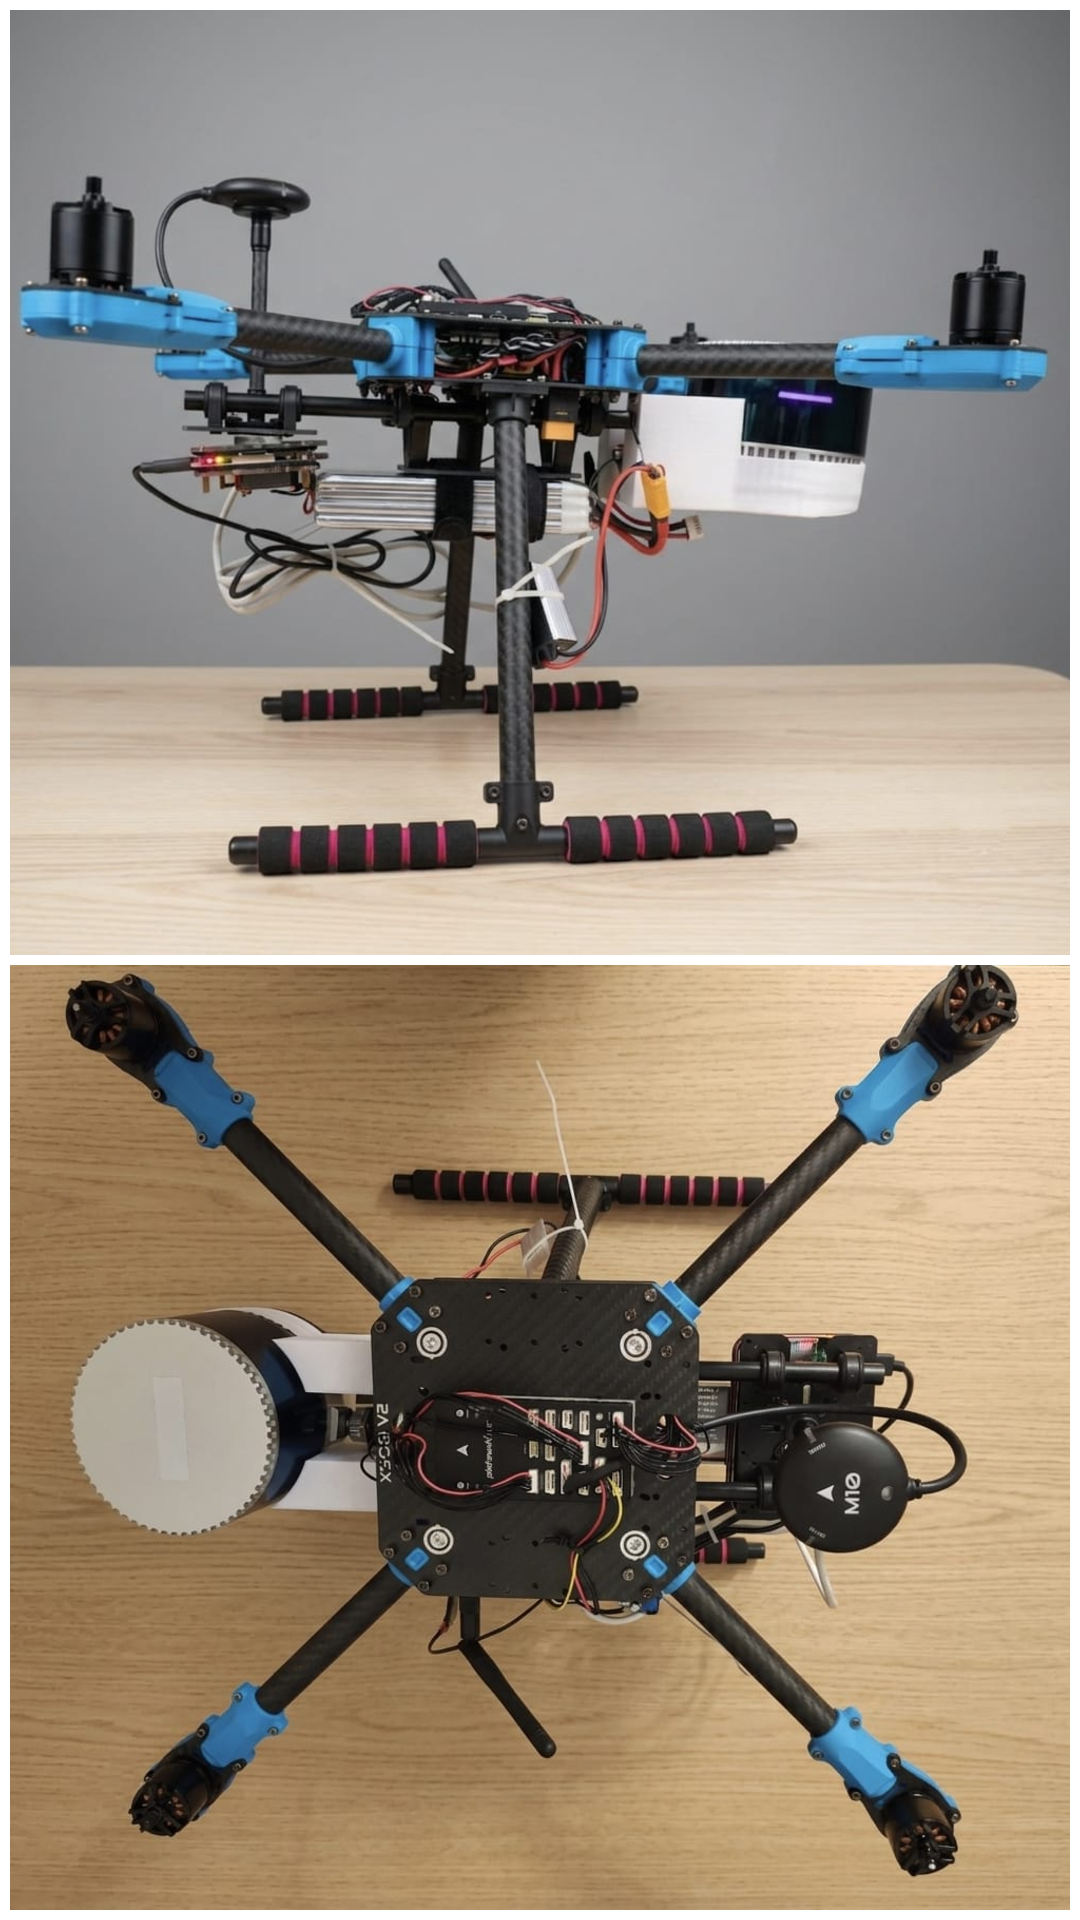
\includegraphics[width=0.5\textwidth]{uav_integration.png}
    \caption{Integrated sensing platform based on the Holybro X500 V2 UAV. The LSLiDAR C16 V4 is mounted on the front of the vehicle using a custom 3D-printed bracket attached to the frame tubes, while the Raspberry Pi is installed underneath the frame on the opposite side to improve weight distribution.}
    \label{fig:uav_integration}
\end{figure}

\section{Data Acquisition System}
\label{sec:data_acquisition}

\subsection{System Architecture}
\label{subsec:system_architecture}

A custom data acquisition pipeline was developed to process the raw measurements generated by the LSLiDAR C16 V4.0 sensor and convert them into structured point cloud representations in PCD format usable in training. Since the sensor transmits data as Ethernet frames containing raw measurement packets, a dedicated software layer is required to decode the incoming information and reconstruct the corresponding three-dimensional points.

The acquisition system is implemented in Python and runs on a computing unit connected to the LiDAR sensor through an Ethernet interface. Python was selected due to its suitability for rapid development and its support for the libraries required by the proposed pipeline, including Scapy for network packet capture, NumPy for numerical processing, and Open3D for point cloud visualization and manipulation. This combination provides the required functionality while facilitating the development and integration of the different processing stages. The system is composed of three main modules: (i) packet capture and parsing, (ii) geometric reconstruction of 3D points, and (iii) real-time visualization and storage of point clouds. These modules correspond directly to the main processing tasks required to transform the raw LiDAR data into usable point cloud representations. Figure~\ref{fig:acquisition_pipeline} illustrates the overall processing pipeline.

The acquisition system is complemented by an offline packet capture and replay module that enables reproducible experiments and system validation without requiring physical access to the LiDAR sensor.


\begin{figure}[htbp]
\centering
\begin{tikzpicture}[
block/.style={
draw,
rectangle,
align=center,
minimum width=3.6cm,
minimum height=1cm
},
arrow/.style={->, thick}
]

% Online path
\node[block] (lidar) {LSLiDAR C16};
\node[block, right=2.8cm of lidar] (network) {Ethernet Traffic};

\node[block, below=1.6cm of network] (parser) {Packet Parser};
\node[block, below=1.6cm of parser] (pcgen) {Point Cloud\\Generation};
\node[block, below=1.6cm of pcgen] (vis) {Open3D Visualization};

% Offline path
\node[block, left=2.8cm of parser] (pcap) {PCAP File\\(Recorded Packets)};
\node[block, below=1.6cm of pcap] (replay) {Packet Replay\\System};

% Arrows online
\draw[arrow] (lidar) -- (network);
\draw[arrow] (network) -- (parser);
\draw[arrow] (parser) -- (pcgen);
\draw[arrow] (pcgen) -- (vis);

% Arrows offline
\draw[arrow] (pcap) -- (replay);
\draw[arrow] (replay) -- (parser);

% Connection note
\node[align=center, below=0.6cm of replay] {\small Same processing pipeline used for both modes};

\end{tikzpicture}
\caption{Online and offline LiDAR data acquisition pipeline with packet capture and replay capability.}
\label{fig:acquisition_pipeline}
\end{figure}

\subsection{Packet Capture and Parsing}
\label{subsec:packet_capture}

Incoming LiDAR data is captured using a network sniffing approach based on the Scapy library.\cite{scapy} The application listens to Ethernet traffic on the dedicated network interface and filters packets originating from the LiDAR sensor IP address. Each packet is processed in real time through a callback function that validates packet size and structure before further processing.

The raw payload is extracted from each Ethernet frame and segmented into structured blocks corresponding to individual laser firings. Each firing contains azimuth information and two distance-intensity return values per channel. The parsing stage decodes the raw binary information into meaningful measurements, including distance and intensity values.

To ensure robustness, validity checks are applied to remove invalid returns, such as zero intensity values or distances outside the sensor operating range.

\subsection{Geometric Reconstruction}
\label{subsec:geometric_reconstruction}

Once the raw measurements are extracted, a module reconstructs three-dimensional points using a polar-to-Cartesian transformation. Each measurement is defined by a distance value and corresponding azimuth and vertical angles, which are converted into Euclidean coordinates using:

\[
x = d \cos(\theta_v) \cos(\theta_a)
\]
\[
y = d \cos(\theta_v) \sin(\theta_a)
\]
\[
z = d \sin(\theta_v)
\]

where \(d\) represents the measured distance, \(\theta_a\) the azimuth angle, and \(\theta_v\) the vertical angle associated with each laser channel.

The software architecture also supports dual echo returns, allowing multiple measurements per laser channel to be processed independently, which increases point density and improves scene representation.

\subsection{Real-Time Point Cloud Streaming}
\label{subsec:streaming}

The reconstructed points are continuously added to a live streaming module implemented using Open3D.\cite{Zhou2018Open3D} A dedicated thread manages real-time visualization, enabling interactive inspection of the acquired environment during data collection. A temporal filtering strategy is applied to remove outdated points based on a time-to-live (TTL) mechanism, ensuring that the visualization reflects only recent sensor measurements.

\subsection{Point Cloud Storage}
\label{subsec:storage}

In parallel with real-time visualization, a dedicated thread periodically stores accumulated point cloud data into disk. A separate thread is responsible for saving the data at fixed time intervals, generating sequential point cloud files in PCD format.\cite{PCDFormat} Each file is timestamped to preserve temporal ordering and facilitate dataset organization.

The resulting dataset consists of a sequence of point clouds representing continuous scans of indoor environments. This dataset forms the basis for subsequent semantic segmentation and human detection experiments described in later sections of this work.

\subsection{Packet Capture and Replay System}
\label{subsec:packet_capture_replay}

In addition to the real-time acquisition pipeline, a dedicated packet capture and replay system was developed to support offline testing and reproducibility of experiments. This module allows LiDAR Ethernet packets to be recorded, stored, and later replayed without requiring access to the physical sensor.

The capture process is implemented using the Scapy library, which listens to incoming Ethernet traffic on the LiDAR network interface. Each packet is stored in PCAP format, preserving the original binary structure of the data.\cite{pcap_format} This approach ensures that no information is lost during the recording process, enabling faithful reproduction of real acquisition scenarios.

Once captured, the recorded packet sequences can be replayed using a custom playback module. During replay, packets are read sequentially from the stored PCAP file and injected into the same processing pipeline used for real-time acquisition. This design ensures that packet parsing, geometric reconstruction, and point cloud generation behave identically in both real-time and offline modes.

A configurable time delay between packets allows the simulation of different acquisition speeds, making it possible to test the robustness of the software under varying temporal conditions. This replay mechanism is particularly useful for debugging, algorithm validation, and controlled experimentation without requiring continuous access to the LiDAR sensor.

Overall, the packet capture and replay system significantly enhances the flexibility of the proposed framework by enabling repeatable experiments and decoupling data acquisition from hardware availability.

\subsection{Modular Design}
\label{subsec:modular_design}

The proposed data acquisition system follows a modular architecture, where each functional component is implemented as an independent module. This design allows different stages of the pipeline to be enabled, disabled, or replaced depending on the specific experimental requirements.

The system is composed of separate modules for packet capture, packet parsing, geometric reconstruction, real-time visualization, data storage, and offline replay. Since these modules communicate through well-defined interfaces, the application can operate in different configurations without modifying the core processing logic.

For example, the real-time visualization module can be disabled when running long-term data collection experiments, while the packet replay module can be used independently for offline testing and debugging. This flexibility improves the usability of the system and facilitates rapid experimentation under different acquisition scenarios.

Overall, the modular design enhances the extensibility and robustness of the pipeline, enabling its adaptation to both real-time UAV deployment and offline dataset generation workflows.

\section{Custom Indoor UAV Dataset Creation}
\label{sec:dataset_creation}

\subsection{Dataset Acquisition Protocol}
\label{subsec:acquisition_protocol}

An indoor LiDAR dataset was collected to evaluate semantic segmentation and human detection under conditions representative of future UAV deployment scenarios. At the current stage of the work, all data were acquired using a static configuration in which the LSLiDAR C16 V4.0 sensor remained fixed during the acquisition process. This setup enabled controlled data collection and facilitated the generation of representative human poses and occlusion conditions.

The dataset was acquired in a laboratory environment containing tables and chairs, providing realistic indoor clutter while maintaining a free central area for the execution of the experiments. Data collection was performed from two different LiDAR viewpoints, obtained by placing the sensor in two distinct positions within the scene. The use of multiple viewpoints introduces variations in visibility, self-occlusion, and point density distribution, partially emulating the viewpoint changes expected during future UAV operation.

A total of 78 valid point clouds were retained, with each point cloud containing approximately 50,000 points. The acquisition protocol initially comprised $4\times4\times4\times2=128$ human-containing configurations, corresponding to four poses, four orientations, four occlusion conditions, and two LiDAR viewpoints, plus four barrier-only reference scenes. After excluding redundant acquisitions in which the subject was completely occluded and therefore provided no additional information, 78 point clouds were retained for the final dataset. Point clouds were generated and stored at fixed acquisition intervals, producing a dataset of independent snapshots suitable for semantic segmentation experiments.


The acquisition protocol was designed to capture a wide range of geometric variations of the human body. Data were collected from a single subject performing several predefined poses, namely standing, sitting, lying down, and a T-pose configuration. These poses were selected to introduce significant variations in body shape, height, and spatial extent, thereby increasing the geometric diversity of the dataset.

To further increase scene complexity, partial occlusions were introduced using two physical barriers of different heights, referred to as the low barrier and the high barrier. Three occlusion configurations were considered: low barrier only, high barrier only, and the simultaneous use of both barriers. These scenarios were designed to reproduce visibility limitations commonly encountered in indoor environments, where furniture, equipment, or structural elements may partially obstruct the view of a person.

For each pose, whenever applicable, the subject was recorded under multiple orientations with respect to the LiDAR sensor. Specifically, acquisitions were performed with the subject facing the sensor and after rotations of (90$^\circ$), (180$^\circ$), and (270$^\circ$). These orientations introduce substantial variations in the observed geometry of the human body and allow the dataset to capture viewpoint-dependent changes in the resulting point clouds.

Although the current dataset has been acquired using a static LiDAR configuration, its design intentionally incorporates variations in pose, orientation, viewpoint, and partial occlusion, providing challenging conditions for evaluating the adaptation of semantic segmentation models to indoor human detection scenarios.
This limitation is considered when interpreting the experimental results, since the dataset does not yet capture the motion-induced variations expected during actual UAV flight.

\begin{figure}[htbp]
\centering
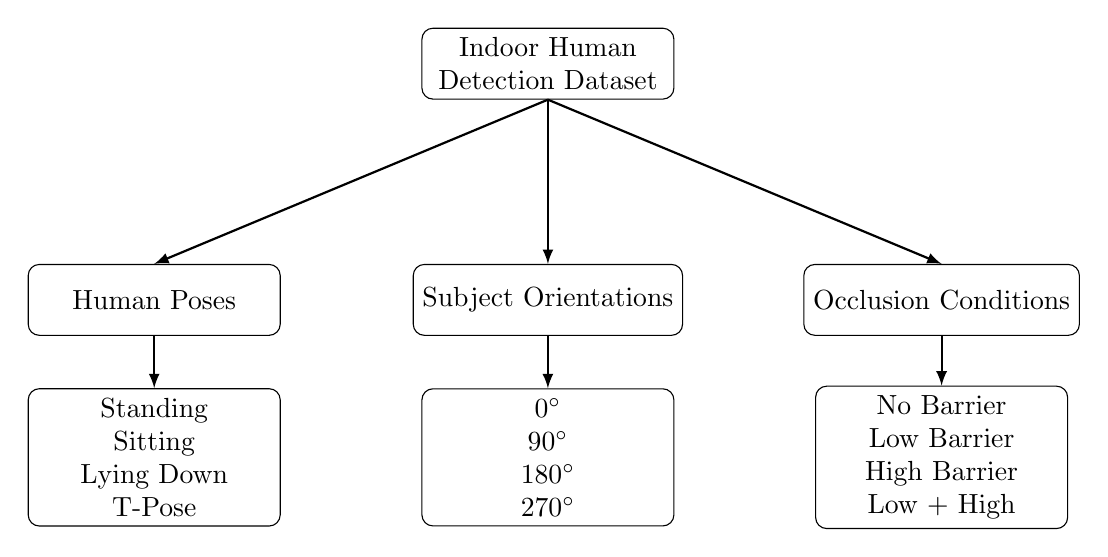
\begin{tikzpicture}[
    every node/.style={
        draw,
        rounded corners,
        align=center,
        minimum width=3.2cm,
        minimum height=0.9cm
    },
    >=latex
]

% Dataset
\node (dataset) at (5,0)
{Indoor Human\\Detection Dataset};

% Titles
\node (pos_title) at (0,-3)
{Human Poses};

\node (ori_title) at (5,-3)
{Subject Orientations};

\node (occ_title) at (10,-3)
{Occlusion Conditions};

% Contents
\node (pos) at (0,-5)
{
Standing\\
Sitting\\
Lying Down\\
T-Pose
};

\node (ori) at (5,-5)
{
$0^\circ$\\
$90^\circ$\\
$180^\circ$\\
$270^\circ$
};

\node (occ) at (10,-5)
{
No Barrier\\
Low Barrier\\
High Barrier\\
Low + High
};

% Connections
\draw[->,thick] (dataset.south) -- (pos_title.north);
\draw[->,thick] (dataset.south) -- (ori_title.north);
\draw[->,thick] (dataset.south) -- (occ_title.north);

\draw[->,thick] (pos_title.south) -- (pos.north);
\draw[->,thick] (ori_title.south) -- (ori.north);
\draw[->,thick] (occ_title.south) -- (occ.north);

\end{tikzpicture}
\caption{Organization of the indoor human detection dataset and the acquisition factors considered during data collection.}
\label{fig:dataset_factors}
\end{figure}

\subsection{Point Cloud Preprocessing}
\label{subsec:pointcloud_preprocessing}

The raw point clouds generated from the LiDAR packets undergo a preprocessing stage before annotation and model training. This stage aims to remove unreliable measurements and reduce the influence of spurious points while preserving the geometric information of the scene.

The first preprocessing step consists of the removal of invalid LiDAR returns during packet decoding. Measurements with zero intensity values or distances outside the valid operating range of the sensor are discarded and are therefore not included in the generated point cloud.

The second filtering stage is applied to remove statistical outliers. During the inspection of the original point clouds, a recurrent cluster of points was observed outside the physical boundaries of the acquisition room. These points corresponded to measurements originating from the exterior of the experimental environment and were therefore considered irrelevant to the indoor scene.

For each point cloud, the Euclidean distance of every point to the sensor origin is computed, and the mean distance ($\mu$) and standard deviation ($\sigma$) of the distribution are estimated. Points whose distance satisfies

\[
|d_i-\mu| > 2\sigma
\]

are considered outliers and are removed from the point cloud. The $2\sigma$ threshold was selected as a simple statistical criterion that effectively removes the distant cluster observed in the original acquisitions while preserving the majority of the points belonging to the indoor scene. This approach provided a simple and computationally inexpensive solution for cleaning the acquired point clouds without requiring manual removal of the unwanted measurements.



\subsection{Point Cloud Annotation}
\label{subsec:annotation}

The collected point clouds required point-wise semantic annotations in order to train and evaluate semantic segmentation models. Since no automatic ground-truth labels were available, a dedicated semi-automatic annotation framework was developed specifically for this work.

The objective of the annotation process was to assign a binary semantic label to each point:

\[
y_i \in \{0,1\},
\]

where \(y_i=1\) denotes points belonging to the \textit{person} class and \(y_i=0\) represents background points.

Manual point-wise annotation of LiDAR data is a highly time-consuming task, particularly when working with dense point clouds containing approximately 50,000 points per acquisition. To reduce the annotation effort while maintaining label quality, an interactive annotation pipeline was implemented using the Open3D library \cite{Zhou2018Open3D}.

The proposed framework follows a semi-automatic workflow. First, the operator manually selects one or more seed points belonging to the human subject using an interactive visualization interface. These seed points are subsequently used to generate an initial segmentation mask through automatic geometric operations. Finally, the generated labels are visually inspected and manually corrected when necessary.

Two complementary annotation strategies were implemented.

The first strategy is based on oriented bounding boxes (OBB). The operator selects several seed points around the target object, and an oriented bounding box is estimated from the selected points. The box is subsequently expanded by a small safety margin and all points located inside the volume are assigned to the \textit{person} class. This approach proved particularly effective for isolated human poses such as standing, sitting, lying down, and T-pose configurations.

The second strategy combines density-based clustering with interactive seed selection. A global DBSCAN segmentation is first performed on the point cloud. The clusters containing the user-selected seed points are then identified and merged to produce an initial human segmentation mask. To prevent the inclusion of distant structures, an additional distance constraint is imposed by limiting the maximum Euclidean distance between candidate points and the selected seeds. Furthermore, a color-based heuristic was introduced to remove floor points that were consistently represented by dark blue intensity values in the visualization colormap. This strategy proved especially useful in partially occluded scenarios and in scenes where the person was connected to surrounding structures.

After the automatic generation of the segmentation masks, all annotations were visually inspected using an interactive preview interface. The operator could accept the proposed labels or repeat the selection process whenever the segmentation was considered unsatisfactory. Minor inaccuracies along object boundaries and occlusion regions were subsequently corrected manually.
\begin{figure}[H]
\centering
\begin{tikzpicture}[
node distance=1.8cm,
every node/.style={
draw,
rounded corners,
align=center,
minimum width=3.5cm,
minimum height=0.9cm
},
>=latex
]

% Main nodes
\node (cloud) {Input Point Cloud};

\node (seed) [below of=cloud]
{Interactive\\Seed Selection};

\node (obb) [below left=2cm and 2cm of seed]
{OBB-Based\\Segmentation};

\node (dbscan) [below right=2cm and 2cm of seed]
{DBSCAN-Based\\Segmentation};

\node (mask) [below=4cm of seed]
{Initial Human Mask};

\node (review) [below of=mask]
{Visual Inspection\\and Validation};

\node (manual) [below of=review]
{Manual Corrections};

\node (labels) [below of=manual]
{Binary Labels\\(\texttt{.npy})};

% Arrows
\draw[->, thick] (cloud) -- (seed);

\draw[->, thick] (seed) -- (obb);
\draw[->, thick] (seed) -- (dbscan);

\draw[->, thick] (obb) -- (mask);
\draw[->, thick] (dbscan) -- (mask);

\draw[->, thick] (mask) -- (review);
\draw[->, thick] (review) -- (manual);
\draw[->, thick] (manual) -- (labels);

\end{tikzpicture}

\caption{Semi-automatic annotation pipeline developed for this work. Human labels are generated through interactive seed selection followed by either OBB-based or DBSCAN-based segmentation and subsequently refined through visual inspection and manual correction.}
\label{fig:annotation_pipeline}
\end{figure}
The final annotations are stored as binary label arrays in NumPy format (\texttt{.npy}), preserving a one-to-one correspondence between the point indices of each point cloud and their semantic labels. This representation simplifies dataset management and allows direct integration with semantic segmentation frameworks during the training stage.

The developed annotation framework is modular and allows different segmentation strategies to be selected depending on the geometric characteristics of the scene. This flexibility considerably reduced the manual annotation effort while maintaining accurate point-wise labels for the human class.



\section{Deep Learning Framework}
\label{sec:deep_learning_framework}
This section describes the deep learning framework adopted for semantic segmentation in this work. First, the selected architectures are presented together with the criteria that motivated their selection. Next, the deployment architecture is described, including the distribution of computation between the onboard embedded platform and an external processing unit. Finally, the training environment used for model development and experimentation is introduced.

\subsection{Selected Architectures}
\label{subsec:selected_architectures}
One of the main objectives of this work is to evaluate the feasibility of deploying deep learning-based semantic segmentation models for indoor UAV perception under edge computing constraints. Consequently, the selection of architectures was guided by three main criteria. First, the models had to operate directly on point clouds without requiring intermediate voxelization or projection steps, preserving the geometric information acquired by the LiDAR sensor. Second, pretrained weights on the Stanford Large-Scale 3D Indoor Spaces (S3DIS) dataset had to be available to enable transfer learning to the proposed UAV dataset. Finally, the selected models had to provide a representative range of computational complexity, allowing the evaluation of the trade-off between segmentation performance and computational requirements.

To satisfy these criteria, six representative point-based architectures were selected. PointNet \cite{Qi2017PointNet} and PointNet++ \cite{Qi2017PointNetPP} were included as baseline models due to their historical relevance and widespread adoption in point cloud semantic segmentation. PointNet established the foundation for directly processing unordered point sets, while PointNet++ introduced hierarchical local feature aggregation, significantly improving segmentation performance.

Dynamic Graph CNN (DGCNN) \cite{Wang2019DGCNN} was selected as a representative evolution of point-based networks. By dynamically constructing neighborhood graphs in the feature space through the EdgeConv operator, DGCNN captures local geometric relationships more effectively than the original PointNet architectures, providing a stronger baseline for comparison.

To evaluate more recent architectures, two variants of PointNeXt \cite{PointNeXt} were considered. PointNeXt-S represents a lightweight configuration specifically suited to efficient inference, making it an attractive candidate for edge computing scenarios where computational resources are limited. In contrast, PointNeXt-XL provides a substantially larger model with higher representational capacity, allowing the analysis of the accuracy gains obtained by increasing model complexity.

Finally, PointVector \cite{PointVector} was included as a modern architecture incorporating vector-based local feature representations. This model extends conventional point-based feature aggregation by explicitly modeling directional geometric information, providing an additional state-of-the-art reference for comparison.

Although other recent point cloud architectures were considered during the model selection process, not all of them were included in the final evaluation. In particular, transformer-based architectures such as Point Transformer were excluded due to their higher computational and training requirements. Preliminary experiments showed that training these models was considerably more demanding and that their inference time was not compatible with the computational constraints considered for the intended edge deployment scenario. Convolution-based architectures were also not prioritized when their computational requirements were expected to be substantially higher than those of the selected point-based models. The final selection therefore focuses on architectures that provide a meaningful range of model complexity while remaining practical for training and inference under the computational constraints of the proposed system.


Together, these architectures span the evolution of point-based semantic segmentation networks, from the original PointNet to more recent large-scale models. At the same time, they cover a broad spectrum of computational requirements, making them particularly suitable for investigating the balance between segmentation accuracy and inference efficiency required for edge computing applications.

Table~\ref{tab:selected_models} summarizes the models considered in this work.

\begin{table}[H]
\centering
\caption{Deep learning architectures selected for evaluation.}
\label{tab:selected_models}
\begin{tabular}{|l|l|l|}
\hline
\textbf{Architecture} & \textbf{Role in this work} & \textbf{Complexity} \\
\hline
PointNet & Baseline architecture & Low \\
\hline
PointNet++ & Improved baseline & Medium \\
\hline
DGCNN & Historical evolution & Medium--High \\
\hline
PointNeXt-S & Lightweight modern model & Medium \\
\hline
PointNeXt-XL & High-capacity modern model & High \\
\hline
PointVector & State-of-the-art reference & High \\
\hline
\end{tabular}
\end{table}

\subsection{Deployment Architecture}
\label{subsec:deployment_architecture}

The initial architecture was designed to deploy the lowest-complexity models directly on the onboard Raspberry Pi, enabling a fully embedded perception pipeline. This approach would allow all data acquisition, processing, and inference tasks to be performed locally on the UAV, minimizing communication latency and eliminating the need for external computing resources.

However, preliminary experiments showed that executing the evaluated deep learning models directly on the Raspberry Pi was not reliable under sustained operation. Although the execution of lightweight architectures was technically possible in principle, the computational load caused significant thermal stress, eventually leading to overheating and automatic system restarts. As a result, a stable and reproducible inference output could not be obtained on the onboard platform. Therefore, onboard deep learning inference was considered impractical for the current hardware configuration.

Consequently, the system architecture was redesigned following a distributed computing approach. In the final implementation, the Raspberry Pi acts exclusively as an onboard acquisition and communication node. Raw LiDAR measurements are received through the Ethernet interface, converted into point cloud representations, and transmitted via a Wi-Fi connection to an external workstation equipped with an NVIDIA GPU. Semantic segmentation inference is then performed on the external computer, where the required computational resources are available.

To enable autonomous operation, a dedicated Linux daemon was developed for the Raspberry Pi. The daemon is automatically executed during system startup and configures the network interface with the static IP address expected by the LiDAR sensor. Once initialized, the acquisition software continuously receives LiDAR packets, reconstructs the corresponding point clouds, and transmits them to a configurable destination IP address over the wireless network.

This design eliminates the need for direct user interaction with the onboard computer. Since all network configuration and acquisition processes are performed automatically, the Raspberry Pi operates as a headless embedded device, requiring no graphical interface, monitor, keyboard, or manual configuration during operation. As a result, the complete sensing system can be powered on and immediately begin transmitting point cloud data to the external processing node.

\begin{figure}[htbp]
\centering
\begin{tikzpicture}[
block/.style={
draw,
rectangle,
align=center,
minimum width=3.8cm,
minimum height=0.9cm
},
arrow/.style={->, thick},
node distance=1.3cm
]

% Nodes
\node[block] (lidar) {LSLiDAR C16 V4};

\node[block, below=of lidar] (eth)
{Ethernet Communication};

\node[block, below=of eth] (rpi)
{Raspberry Pi\\
Acquisition Node};

\node[block, below=of rpi] (wifi)
{Wi-Fi Communication};

\node[block, below=of wifi] (gpu)
{External Workstation\\
CUDA-enabled GPU};

\node[block, below=of gpu] (seg)
{Semantic Segmentation};

% Arrows
\draw[arrow] (lidar) -- (eth);
\draw[arrow] (eth) -- (rpi);
\draw[arrow] (rpi) -- (wifi);
\draw[arrow] (wifi) -- (gpu);
\draw[arrow] (gpu) -- (seg);

% Side notes
\node[align=left,right=2.8cm of rpi,font=\small]
{
\textbf{Onboard}\\
Automatic daemon\\
Static IP configuration\\
Point cloud generation
};

\node[align=left,right=2.8cm of gpu,font=\small]
{
\textbf{External}\\
CUDA acceleration\\
Deep learning inference\\
Model execution
};

\end{tikzpicture}

\caption{Deployment architecture adopted in this work. LiDAR measurements are transmitted via Ethernet to the Raspberry Pi, where point clouds are reconstructed and subsequently sent through Wi-Fi to an external GPU-equipped workstation for semantic segmentation.}
\label{fig:deployment_architecture}
\end{figure}

\subsection{Point Cloud Reception and Inference}
\label{subsec:receiver_inference}

The external processing stage is implemented through a dedicated point cloud receiver and inference module. These components provide the interface between the point cloud stream transmitted by the onboard Raspberry Pi and the trained semantic segmentation models executed on the external workstation. The receiver operates as a TCP server, listening on a configurable network port for incoming point cloud data from the acquisition node.

For each received point cloud, the communication protocol first transmits a four-byte header containing the number of points in the frame. The receiver subsequently reads the corresponding point data as 32-bit floating-point values and reconstructs the point cloud as an $(N\times3)$ array containing the \textit{XYZ} coordinates of each point. Once the complete point cloud has been received, it is passed directly to the inference module for processing. This communication mechanism provides a simple interface between the acquisition and processing stages while allowing the two components to operate independently.

The inference stage is implemented through an \texttt{InferenceEngine} that loads the selected trained model and manages the execution of the prediction process. The received point cloud is first converted to the numerical representation expected by the network and prepared as a batched input containing the three-dimensional coordinates of the points. The processed input is then forwarded through the selected segmentation model, which produces point-wise class scores. The predicted semantic class for each point is obtained by selecting the class with the highest output score, resulting in a binary prediction corresponding to either the \textit{Human} or \textit{Background} class.

The inference module is designed to support the execution of the trained segmentation models independently of the data acquisition process. This separation allows the same inference software to be used with both live point clouds transmitted by the UAV and previously recorded data, facilitating model evaluation and controlled experiments. The inference engine also performs an initial warm-up stage before performance measurements are collected, reducing the influence of initialization effects on the reported inference times.

For each processed point cloud, the inference module records the processing time associated with the model execution and computes the corresponding segmentation metrics when ground-truth labels are available. These measurements provide the basis for evaluating the computational performance of the deployed models and are reported together with the segmentation results in the experimental evaluation.


\subsection{Training Environment}
\label{subsec:training_environment}

All model training and fine-tuning experiments were performed on a laptop equipped with an NVIDIA GeForce RTX 4050 GPU with CUDA acceleration. The software environment was based on Python and the PyTorch deep learning framework, providing GPU-accelerated training and inference for all evaluated architectures.

To ensure a fair comparison between models, a common training framework was adopted whenever possible. PointNeXt, DGCNN, and PointVector were trained using the OpenPoints framework, which provides unified implementations of state-of-the-art point cloud processing architectures. Using a common implementation minimizes differences arising from software design choices and allows the comparison to focus on the intrinsic characteristics of each network architecture.

PointNet and PointNet++ were trained using their official PyTorch implementation. This decision was motivated by the original objective of deploying these lightweight architectures directly on the Raspberry Pi. Unlike OpenPoints, whose implementation relies on CUDA for efficient execution, the official PyTorch implementation can be executed on CPU-only platforms, making it more suitable for evaluating the feasibility of onboard inference on the embedded system. Although the final system adopted a distributed deployment architecture, the official implementation was retained throughout the development process.

Minor modifications were introduced to both codebases to support the proposed transfer learning workflow. In particular, the input layer of each network was adapted to process point clouds containing only three-dimensional coordinates (\textit{XYZ}). The pretrained models available for the S3DIS dataset expect six-dimensional input features, consisting of spatial coordinates (\textit{XYZ}) and color information (\textit{RGB}). As the LSLiDAR C16 sensor does not provide color measurements, the networks were modified to accept only the geometric information while preserving the remaining pretrained weights.

This unified software environment enables the evaluation of different point cloud segmentation architectures under comparable training conditions while requiring only minimal adaptations to accommodate the characteristics of the proposed UAV LiDAR dataset.

\begin{table}[H]
\centering
\caption{Training environment used in this work.}
\label{tab:training_environment}
\begin{tabular}{|l|l|}
\hline
\textbf{Component} & \textbf{Specification} \\
\hline
Operating System & Ubuntu 22.04 LTS \\
Python & 3.10.22 \\
Deep Learning Framework & PyTorch 2.5.1 \\
GPU & NVIDIA GeForce RTX 4050 \\
CUDA & CUDA Toolkit 12.2 \\
Framework & OpenPoints (PointNeXt, DGCNN, PointVector) \\
Official Implementations & PointNet, PointNet++ \\
\hline
\end{tabular}
\end{table}

\section{Transfer Learning Strategy}
\label{sec:transfer_learning}

\subsection{Pretraining on S3DIS}
\label{subsec:pretraining_s3dis}


Training deep neural networks for point cloud semantic segmentation requires large amounts of annotated data. However, manually labeling three-dimensional point clouds is a time-consuming and labor-intensive process, making it impractical to train complex models from scratch using the proposed UAV dataset alone. To overcome this limitation, a transfer learning strategy was adopted by initializing each network with weights pretrained on the Stanford Large-Scale 3D Indoor Spaces (S3DIS) dataset \cite{Armeni2016S3DIS}.

The S3DIS dataset is one of the most widely used benchmarks for indoor semantic segmentation and contains densely annotated point clouds acquired from office buildings, conference rooms, corridors, and other indoor environments. Since the environments represented in S3DIS share geometric characteristics with the indoor scenarios considered in this work, pretrained models provide a suitable initialization for subsequent adaptation to the custom UAV dataset.

For PointNeXt, DGCNN, and PointVector, the pretrained checkpoints provided by the OpenPoints framework were employed. These models were originally trained following the standard Area~5 evaluation protocol of S3DIS, which is commonly adopted as the benchmark for indoor semantic segmentation.

In contrast, PointNet and PointNet++ were pretrained using their official PyTorch implementation. As compatible pretrained weights were not available for the required implementation, both networks were trained from scratch on the complete S3DIS training split, using the corresponding validation split for model selection. The resulting checkpoints were then used as the initialization for the transfer learning stage.

By initializing all architectures from pretrained weights instead of random parameters, the networks already encode meaningful geometric representations before being exposed to the custom UAV dataset. This significantly reduces the amount of task-specific data required for training, accelerates convergence during optimization, and generally improves the final segmentation performance compared to training from scratch.

\subsection{Fine-Tuning on the Custom UAV Dataset}
\label{subsec:fine_tuning}

Following the pretraining stage, all selected architectures were adapted to the proposed UAV LiDAR dataset through a full fine-tuning strategy. The objective was to transfer the geometric representations learned from the S3DIS dataset to the binary semantic segmentation task considered in this work while preserving as much pretrained knowledge as possible. The original pretrained models were designed to process six-dimensional point features composed of three-dimensional coordinates (\textit{XYZ}) and color information (\textit{RGB}). Since the LSLiDAR C16 sensor provides only geometric information, the input layer of each network was modified to accept three-dimensional input features corresponding exclusively to the spatial coordinates of each point. As a consequence, the weights associated with the modified input layer were randomly initialized, while all remaining compatible parameters were loaded directly from the pretrained models. Similarly, the original segmentation heads were designed to predict the semantic classes defined by the S3DIS dataset. To adapt the networks to the proposed binary segmentation problem, the final classification layer of each architecture was replaced with a new output layer containing two classes: \textit{Human} and \textit{Background}. Since the dimensions of the original and target classification layers differ, the new segmentation heads were also initialized with random weights. After these architectural modifications, all networks were trained using a full fine-tuning strategy. Unlike feature extraction approaches, where part of the network remains frozen, all layers were allowed to update during optimization. This enables the pretrained geometric representations to progressively adapt to the characteristics of the UAV LiDAR data while simultaneously learning the new binary classification task. The resulting transfer learning strategy preserves the majority of the pretrained knowledge acquired from S3DIS while adapting the input representation and output prediction layers to the characteristics of the proposed dataset. This approach provides a suitable compromise between efficient training and effective domain adaptation, particularly considering the limited size of the custom UAV dataset.

\begin{figure}[H]
\centering
\begin{tikzpicture}[
block/.style={
draw,
rectangle,
align=center,
minimum width=4.2cm,
minimum height=0.9cm
},
arrow/.style={->, thick},
node distance=1.4cm
]

% Nodes
\node[block] (pretrained)
{Pretrained Model\\
(S3DIS)};

\node[block, below=of pretrained] (input)
{Input Layer Adaptation\\
XYZRGB $\rightarrow$ XYZ};

\node[block, below=of input] (head)
{Segmentation Head Replacement\\
13 Classes $\rightarrow$ 2 Classes};

\node[block, below=of head] (weights)
{Load Compatible\\
Pretrained Weights};

\node[block, below=of weights] (finetune)
{Full Fine-Tuning\\
(All Layers Trainable)};

\node[block, below=of finetune] (final)
{Fine-Tuned Model\\
(Custom UAV Dataset)};

% Arrows
\draw[arrow] (pretrained) -- (input);
\draw[arrow] (input) -- (head);
\draw[arrow] (head) -- (weights);
\draw[arrow] (weights) -- (finetune);
\draw[arrow] (finetune) -- (final);

% Notes
\node[right=3cm of input,align=left,font=\small]{
\textbf{Modified}\\
Random initialization
};

\node[right=3cm of head,align=left,font=\small]{
\textbf{Modified}\\
Random initialization
};

\node[right=3cm of weights,align=left,font=\small]{
\textbf{Reused}\\
All compatible layers
};

\node[right=3cm of finetune,align=left,font=\small]{
\textbf{Training}\\
No frozen layers
};

\end{tikzpicture}

\caption{Transfer learning strategy adopted in this work. The pretrained models are adapted by modifying the input layer and segmentation head, while all compatible pretrained weights are retained. The complete network is then fine-tuned on the proposed UAV dataset.}
\label{fig:transfer_learning_strategy}
\end{figure}

\subsection{Training Configuration}
\label{subsec:training_configuration}

To ensure a consistent comparison between the selected architectures, a common training protocol was adopted for all experiments. The training configuration was designed considering the limited size of the custom UAV dataset, the strong class imbalance between human and background points, and the computational constraints of the available GPU.

Each model was trained for a maximum of 100 epochs using the AdamW optimizer. The maximum number of epochs was selected to provide sufficient training time for the models to converge while avoiding unnecessarily long training runs. Since the optimal number of epochs may vary between architectures, an early stopping strategy was employed based on the validation mean Intersection over Union (mIoU). Training was terminated if no improvement in validation mIoU was observed for 20 consecutive epochs. The model achieving the highest validation mIoU was retained for subsequent evaluation.

The AdamW optimizer was selected as a robust optimization method for fine-tuning pretrained neural networks. In particular, its decoupled weight decay provides an additional regularization mechanism that is useful when adapting models to a relatively small target dataset. The initial learning rate was set according to the recommendations of the corresponding implementation for each architecture, rather than enforcing a single value across frameworks with different optimization settings. A ReduceLROnPlateau scheduler was used to reduce the learning rate when validation performance stopped improving, allowing the optimization process to continue with smaller parameter updates during later stages of training.

A batch size of eight point clouds was used for all experiments. This value was selected as a compromise between GPU memory consumption and training stability, considering the different memory requirements of the evaluated architectures. Each input sample contained 4096 points. This fixed number provides a consistent input size across architectures while keeping the computational and memory requirements manageable for the available GPU.

The Cross-Entropy loss function was used as the optimization objective, as the task is formulated as point-wise binary semantic classification between the \textit{Human} and \textit{Background} classes. No architecture-specific loss functions were introduced, allowing the comparison to focus on differences between the segmentation models rather than differences in the optimization objective.

Data augmentation was applied during training to reduce overfitting and improve the robustness of the models to variations expected in UAV-based LiDAR observations. The applied transformations included random rotations around the vertical ($z$) axis, random scaling, random translations, coordinate jittering, and random point dropout. These transformations were selected to reproduce variations in sensor viewpoint, object position, point distribution, and measurement density without altering the semantic identity of the human instances.

Since the proposed dataset contains substantially more background points than human points, a sampling strategy was introduced to increase the frequency with which human-containing regions were presented during training. Specifically, 70\% of the training samples were generated using class-aware sampling, while the remaining 30\% were obtained through standard random sampling. The class-aware component increases the probability of observing regions containing human points, reducing the risk that the optimization process becomes dominated by the background class. The random component was retained to preserve samples representative of the natural point distribution of the scenes. The 70/30 ratio was therefore chosen as a compromise between increasing the representation of the minority class and maintaining the original scene distribution.

Because the sampling procedure is performed online, the selected points are recomputed during training rather than using a fixed set of subsampled point clouds. Consequently, different subsets of the original point clouds can be presented to the network across epochs, providing an additional source of variation during training.

The complete training configuration adopted throughout this work is summarized in Table~\ref{tab:training_configuration}.

\begin{table}[H]
\centering
\caption{Training configuration used for all fine-tuning experiments.}
\label{tab:training_configuration}
\begin{tabular}{|l|l|}
\hline
\textbf{Parameter} & \textbf{Value} \\
\hline
Maximum epochs & 100 \\
Early stopping & 20 epochs (validation mIoU) \\
Batch size & 8 \\
Optimizer & AdamW \\
Initial learning rate & Recommended for each architecture \\
Learning rate scheduler & ReduceLROnPlateau \\
Weight decay & Enabled \\
Loss function & Cross-Entropy Loss \\
Input points & 4096 \\
Sampling strategy & 70\% Class-aware / 30\% Random \\
Data augmentation & Rotation (Z), Scaling, Translation, Jitter, Point Dropout \\
Model selection & Best validation mIoU \\
\hline
\end{tabular}
\end{table}